\documentclass[16pt]{beamer}
\usepackage{algorithm}
\usepackage{algorithmic}
\usepackage[numbers]{natbib}
\usepackage{pgf,pgfarrows,pgfnodes}
% \usepackage{beamerthemesplit} // Activate for custom appearance

\title{Bayesian nonparametric discrete sequence models and the goal of developing general-purpose predictive models}
\author{Frank Wood \\\qquad \\ joint work with Nicholas Bartlett, David Pfau, Jan Gasthaus, C\'{e}dric Archambeau, Lancelot James, Yee Whye Teh, and more...}
\date{\today}



\usetheme{Darmstadt}
%\usetheme{Copenhagen}
%\usefonttheme[onlylarge]{structurebold}
%\setbeamerfont*{frametitle}{size=\normalsize,series=\bfseries}
%\setbeamertemplate{navigation symbols}{}

\usepackage{amsfonts}
\usepackage{amsmath}
%\newcommand{\argmax}{\operatornamewithlimits{argmax}}
\def\newblock{\hskip .11em plus .33em minus .07em}
% Setup TikZ

\newcommand{\ubf}{\mathbf{u}}
\newcommand{\xbf}{\mathbf{x}}
\newcommand{\sbf}{\mathbf{s}}
\newcommand{\py}{\mathcal{PY}}
\newcommand{\vbf}{\mathbf{v}}
\newcommand{\Prob}{\mathrm{P}}
\newcommand{\Psmooth}{\Prob_\text{smooth}}
\newcommand{\parent}{\pi}
\newcommand{\suffix}{\sigma}
\newcommand{\UHPYP}{SM}
\newcommand{\PLUMP}{PLUMP}
\newcommand{\Oh}{\mathcal{O}}
\newcommand{\tree}{\mathcal{T}}

% \newcommand{\cusk}{c_{\ubf s k}}
% \newcommand{\cus}{c_{\ubf s \cdot}}
% \newcommand{\cu}{c_{\ubf \cdot \cdot}}
% \newcommand{\tus}{t_{\ubf s}}
% \newcommand{\tu}{t_{\ubf \cdot}}
\newcommand{\cusk}{c_{\ubf s k}}
\newcommand{\cus}{c_{\ubf s}}
\newcommand{\cu}{c_{\ubf \cdot}}
\newcommand{\tus}{t_{\ubf s}}
\newcommand{\tu}{t_{\ubf \cdot}}
\newcommand{\cset}{\{\cusk\}_{s\in \Sigma,k \in \{1,\ldots,t_{\ubf s}\}}}
\newcommand{\tset}{\{\tus\}_{s\in \Sigma}}
\newcommand{\bydef}{\equiv}
\newcommand{\state}{\mathcal{S}_{\xbf}}
\newcommand{\statei}{\mathcal{S}_{\xbf_{1:i}}}
\newcommand{\emptystring}{\varepsilon}
\newcommand{\gcount}{\hat{c}}
\newcommand{\escape}{\mathtt{esc}}

\newcommand{\todo}[1]{\begin{center}\textbf{TODO: } #1 \end{center}}
\newcommand{\figref}[1]{\figurename~\ref{#1}}
\newcommand{\predictive}{\Prob(x_i|\xbf_{1:i-1})}
\newcommand{\ywcomment}[1]{\textbf{#1}}
\newcommand{\jgcomment}[1]{ { \textcolor{red}{#1} } }




\title[Sequence Memoizer] 
{
	Bayesian nonparametric discrete sequence modeling and the goal of general-purpose predictive models
}

\author[http://www.stat.columbia.edu/$\sim$fwood]
{
  Frank~Wood \\ 
 \qquad \\
  {\small joint work with \\ \qquad \\ Nicholas Bartlett, David Pfau, Jan Gasthaus, C\'{e}dric Archambeau, Lancelot James, Yee Whye Teh, and more...}
}

\institute[Columbia University]
{
  %\inst{1}%
  Columbia University
}

%\def\blfootnote{\xdef\@thefnmark{}\@footnotetext}

% The main document

%\setbeamertemplate{framefooter}{ 
%\begin{centering} 
%\large{\insertframetitle} \\
%\small{\insertframesubtitle}
%\par 
%\end{centering} 
%} 


\begin{document}
\frame{\titlepage}


\section{Setup}
\subsection{Goal }
\frame[t] {
\begin{itemize}
\item Actors in the world must have predictive models of the world in order to act efficiently
\item Better predictive models yield better plans and more rewarding sequences of actions
\item Biological organisms
\begin{itemize}
\item observe sequences of binary vectors
\item build predictive models of the world
\item output sequences of binary vectors
\end{itemize}
\end{itemize}
Ultimate goal: learner capable of generalizing well (predictive performance) given a sequence of discrete observations from the world.
}

\subsection{Compression }
\begin{frame}[t]{}
Any predictive model can be used to compress observation sequences
\begin{itemize}
\item Shannon established a direct connection between compression and probabilistic modeling \cite{Shannon1948}.
\item Compression performance measured in {\em bits}, {\em log-loss} (bits per byte), or {\em perplexity} instead of likelihood or evidence.
\item Units allow comparison between human, deterministic algorithms, and probabilistic models.
\end{itemize}
\end{frame}	


\subsection{Predictive modeling for planning and streaming compression have the same computational requirements}
\begin{frame}[t]{}
Computational requirements for predictive model
\begin{itemize}
\item Incremental model estimation given a single observation sequence of growing (unbounded) length
\item Estimator must have worst case linear time complexity
%\begin{itemize}
%\item Joint because we want all marginal and conditional distributions
%\item Single observation because we only see a single data ``stream.''
%\end{itemize}
\item The model must be representable in worst case constant space
\item Predictive inference must be performed in worst case constant time
\end{itemize}


%\begin{alertblock}{Nature of Problems}
%Computational
%\end{alertblock}
\end{frame}	

%\section{Intuition}
%\section[Outline]{}
%\frame[t]{\tableofcontents}
\subsection{Sequence of discrete observations from an arbitrary stochastic process}
\frame[t]{
\begin{block}{Binary sequence (model definitions)}
\[
\begin{array}{l}
0,1,0,0,1,0,0,1...
\end{array}
\]
\end{block}
%\frametitle{Sequential Discrete Observations}
\begin{block}{Byte sequence  (compression experiments)}
\[
\begin{array}{l}
01001001 , 01101110 , 00100000 , 01110100,\\
01101000 , 01110010 , 01100101 , 01100101,\\
%00100000 , 01100100 , 01100001 , 01111001,\\
%01110011 , 00100000 , 01111001 , 01101111,\\
%01110101 , 01110010 , 00100000 , 01101000,\\
%01100001 , 01110010 , 01100100 , 00100000,\\
%01100100 , 01110010 , 01101001 , 01110110,\\
%01100101 , 00100000 , 01110111 , 01101001,\\
01101100 , 01101100 , 00100000 , 01100011,\\
01110010 , 01100001 , 01110011 , 01101000\ldots
\end{array}
\]
\end{block}

\begin{block}{Abitrary-ary sequence (language modeling, future work)}
\[
\begin{array}{l}
0101 , 0110111000100000 , 00100,\\
00 , 01110 , 011001001100101,\\
%00100000 , 01100100 , 01100001 , 01111001,\\
%01110011 , 00100000 , 01111001 , 01101111,\\
%01110101 , 01110010 , 00100000 , 01101000,\\
%01100001 , 01110010 , 01100100 , 00100000,\\
%01100100 , 01110010 , 01101001 , 01110110,\\
%01100101 , 00100000 , 01110111 , 01101001,\\
%01101100 , 01101100 , 00100000 , 01100011,\\
01110010 01100001 01110011, 1\ldots
\end{array}
\]
\end{block}

}



%\subsection{General-purpose predictive modeling assumptions and requirements}
%\begin{frame}[t]{}
%Requirements
%\begin{itemize}
%\item Incrementally estimate a large set of (or all) conditional distributions ($G$) in worst case time linear in the length of an unbounded sequence of observations.
%\item Represent the model in worst case constant space.
%\item Do predictive inference in worst case constant time.
%\end{itemize}
%Nature's assumptions
%\begin{itemize}
%\item Shortness is preferred
%\item Recency matters
%\item Power-laws permeate
%\end{itemize}
%\end{frame}	

\subsection{One way to do this: i.i.d. conditional distributions; introduction to notation}
\begin{frame}[t]{}
Let $\Sigma$ be a set of symbols, let $\x = x_1, x_2, ..., x_T$ be an observed sequence, $x_t,s,s'  \in \Sigma$, and $\context \in \W = \{\w_1, \w_2, \ldots \w_K\}$ with $\w_k \in \Sigma^+$. 
\begin{align*}
G_\context(s)=\frac{N(\context s)}{\sum_{s'\in\Sigma}N(\context s')}\label{eqn:mll}
\end{align*}
is the maximum likelihood estimator for the conditional distribution ${P}(X=s|\context) \equiv G_\context(s)$.
\vspace{.5cm}

Estimating a finite set of conditional distributions corresponding to a finite set of ``contexts'' $\context$ generally yields a poor model.  Why?

\begin{itemize}
\item Long $\context$'s often have few counts
\item   Maximum likelihood overconfident.
\item   Finite set of contexts might miss important contexts.
\end{itemize}

%\vspace{.5cm}
%Note: first stochastic memoization rule.  Only those $s$'s seen before returned.

\end{frame}	





\begin{frame}[t]{}
What are the``states'' of this model?
\begin{itemize}
\item States are explicit and observable, one per context $\u$.
\item Predictions are made per state.
\item ``Transitions'' from state to state given an emission are deterministic 
\[\delta(\u,s) =  \argmax_k u_{n-k}u_{n}s \in \W \]
\end{itemize}
No "sharing" of statistical strength between states; poor generalization.
\end{frame}

\subsection{Can do better: Bayesian regularization}
\begin{frame}[t]{}
Can treat $G$'s as random and integrate them out
\begin{align*}
P(x_{T+1}=s|\x= \u) = \int P(x_{t+1}=s|G_\context)P(G_\context|\data)dG = {\EE[G_\context(s)] } ,
\end{align*}
yielding, for instance,
\begin{align*}
\EE[G_\context(s)]=\frac{N(\context s) + \frac{\alpha}{|\Sigma|}}{\sum_{s'\in\Sigma}N(\context s') + \alpha}
\end{align*}
in the case of independent Dirichlet priors, i.e.
\vspace{-.5cm}
\begin{center}
\begin{eqnarray*}
G_\context &\sim& \Dir(\frac{\alpha}{|\Sigma|}) \\
x_t | x_{t-k},\ldots,x_{t-1} = \context &\sim& G_\context
\end{eqnarray*}
\end{center}
Same ``states,'' prior makes each estimate more conservative.

%\vspace{.5cm}
%Note: new stochastic memoization rule.  Unobserved $\sigma$'s can be returned.  Good values of $\alpha$ can improve predictive performance.

\end{frame}

\subsection{Share statistical strength between related world states: hierarchical Bayes (i.e.~Hierchical Dirichlet Process (HDP) \cite{Teh2006b})}
  \frame[t] {%slide 9
Can relate $G_\context$ to a related distribution $G_\parent$ (more than one possible) where, for instance, $\sigma(x_1x_2x_3\ldots x_t) = x_2x_3\ldots x_t$ could be the suffix operator
\[\EE[\G_\context(s)]
= \EE\left[
\frac{N(\context s)+ \alpha \G_\parent(s)}{\sum_{s'\in\Sigma} N(\context s') + \alpha}\right]
\]
Where now the counts (latent variables)
\[\{N(\ubf's')\}_{\ubf'\in\Sigma^+, s'\in\Sigma}\] along with $\alpha$, must be marginalized, typically by Monte Carlo methods.

\vspace{.5cm}
%Note: stochastic memoizer now can return unobserved $\sigma$'s in the context $\context$ {\em and} the probability of returning any given symbol is affected by the probability of it being returned by other, related contexts.
%\vspace{.25cm}\newline
More states ($\u \in \Sigma^+$) but potentially better predictive distribution estimates.
}






 %for DP's and PYP's we will sample directly from $P(x_{i+1} | \xbf_{1:i})$ given a marginalized representation of the hierarchy $\GG$ consisting of counts 
 %\[P(x_{i+1} | \xbf_{1:i}) \approx \frac{1}{L}\sum_{\ell = 1}^L P(x_{i+1} | \xbf_{1:i}, \GG_\ell), \; \GG_\ell \sim P(\GG | \xbf_{1:i})\]

 

 % \frame[t] {%slide 9
%\begin{align}
%\label{eq:predictive}
%P(x_{T+1}=s|\data) = \int P(x_{T+1}=s|G)P(G|\data)dG = {\EE[G(s)] } ,
%\end{align}
% }




\section{Sequence Memoizer}



\subsection{Sequence Memoizer}
\frame[t] {
Is it possible to simultaneously estimate predictive distributions for all ``states'' in such a model?
\vspace{.5cm}
\begin{block}{Sequence memoizer (SM), \citet{Wood2011}}
The SM is a compactly-representable, unbounded-depth, hierarchical, Bayesian-nonparametric prior over discrete sequence distributions for which incremental Bayesian updating and predictive inference is efficient.
\end{block}
\begin{block}{Graphical Pitman-Yor process (GPYP), \citet{Wood2008a}}
The GPYP is tool for graphical model structure learning.  Using it, which generalizations are important for each predictive state in the model can be learned.
\end{block}
}

 \subsection{Notation}
 \frame[t] {%slide 8
 Let $\GG = \{\G_{\context}\}, \forall \context \in \Sigma^+$ be {\em all} conditional distributions over a countable alphabet $\Sigma$ and $\xbf = x_1, x_2, \ldots, x_i, \ldots \in \Sigma^+$ be a sequence of discrete observations. The joint distribution of $\xbf$ and $\GG$ is
\begin{eqnarray*}
P(\xbf,\GG) &=& P(\GG)P(\xbf|\GG) \nonumber \\
P(\xbf,\GG) &=& P(\GG)\prod_{t=0}^{|\xbf|-1}G_{\xbf_{1:t}}(x_{t+1})
\end{eqnarray*}
Expanding $P(\xbf|\GG)$ makes shows
\begin{align}
P(\xbf|\GG) = G_{\varepsilon}(x_{1})G_{x_1}(x_{2})G_{\xbf_{1:2}}(x_{3})\cdots G_{\xbf_{1:(|\xbf|-1)}}(x_{|\xbf|})  \nonumber 
\end{align}
that this is the joint\footnote{$P(x_1,\ldots,x_T|\theta) = P(x_1|\theta) P(x_2 | x_1, \theta) P(x_3 | x_1,x_2, \theta) \cdots P(x_T | \xbf_{1:(T-1)}, \theta)$} distribution of $\xbf$. The prior $P(\GG)$ directly regularizes the joint distribution itself.  


 }



 \subsection{Sketch of sequence memoizer inference}
  \frame[t] {%slide 9
Bayesian inference
\begin{itemize}
\item Prediction
 \[P(x_{T+1}=s | \xbf) = \int P(x_{T+1}=s | \GG) dP(\GG | \xbf) = \EE[\G_\context(s)] \]
 where $\context = \xbf_{1:t}$.
\item Posterior updating (sketch)
\[P(\GG|\data) \propto P(x_T | \GG) P(\GG | x_{1:(T-1)})\]

\end{itemize}
}



\subsection{(Binary) sequence memoizer = (binary) hierarchical PY process \cite{Teh2006a} of unbounded depth.}

  \frame[t] {%slide 27
 %\frametitle{A Way to Tie Together ``Related'' Conditional Distributions}
 \begin{figure}[htbp]
\begin{center}
%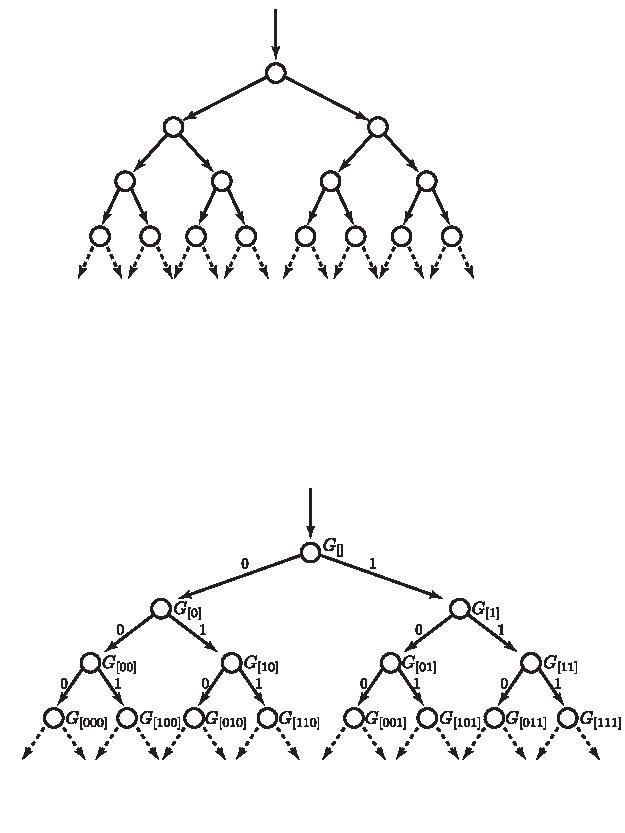
\includegraphics[trim = 4cm 8cm 4cm 8cm, clip, width=5cm]{jtfig/base.pdf}
\vspace{2cm}
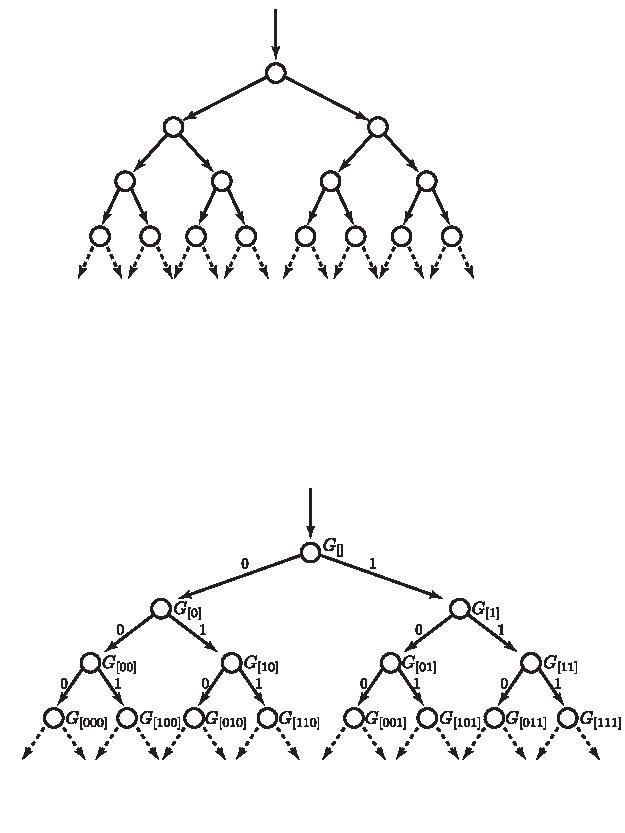
\includegraphics[trim = 2cm 2cm 2cm 10cm, width=8cm]{jtfig/base.pdf}
%\caption{Test perplexity vs.~number of training observations.}
\label{fig: gm_binary_complete}
\end{center}
\end{figure}
}

\subsection{Pitman-Yor process}
\frame[t] {
%\frametitle{Pitman Yor Process (PYP) : Definition \cite{Pitman1997a}}
 A Pitman-Yor process $\PY(c,d,H)$ is a distribution over distributions with three parameters
\begin{itemize}
\item A discount $ 0 \le d < 1 $ that controls power-law behavior
\begin{itemize}
\item $d=0$ is Dirichlet process (DP)
\end{itemize}
\item A concentration $c > -d$ like that of the DP
\item A base distribution $H$ also like that of the DP
\end{itemize}
\vspace{.25cm}
Key properties (more to come): \newline

If $G\sim\PY(c,d,H)$ then {\em a priori}

\begin{itemize}
\item $\EE[G(s)] = H(s)$
\item $\Var[G(s)] = (1-d)H(s)(1-H(s))$
\end{itemize}

}

\subsection{Binary sequence memoizer}
  \frame[t] {%slide 27
  Notation
% \frametitle{Sequence Memoizer, \citet{Wood2009}}
\begin{eqnarray*}
	\G_{\varepsilon} | \U_{\Sigma}, d_0 &\sim& \PY(d_0, 0, \U_{\Sigma }) \\
		\G_{\bf{u}} | \G_{\sigma(\bf{u})}, d_{|\bf{u}|} &\sim& \PY(d_{|\bf{u}|}, 0, \G_{\sigma(\bf{u})}) \hspace{.35cm} \forall {\bf u} \in \Sigma^+\\
	x_t | x_1,  \ldots, x_{t-1} = \bf{u} &\sim& \G_{\bf{u}}
\end{eqnarray*}
Here $\sigma(x_1x_2x_3\ldots x_t) = x_2x_3\ldots x_t$ is the suffix operator, $\Sigma = \{0,1\}$, and $\U_{\Sigma } = [.5, .5] $.
\bigskip

Nature's assumptions
\begin{itemize}
\item Shortness assumption encoded by implicit geometric sequence length distribution
\item Recency assumption encoded by form of coupling related conditional distributions (``back-off'')
\item Power-law effects encoded by the choice of hierarchical modeling glue: the Pitman-Yor process (PY).
\end{itemize}


}

% \frame[t] {%slide 27
% \frametitle{Sequence Memoizer, \citet{Wood2009}}

%\begin{align}
%\prob_\varepsilon &\sim \py(\disc_0,\prob_0)  \label{eqn:hierbayes}\\
%\prob_\context|\prob_\parent &\sim \py(\disc_{|\context|},\prob_\parent) &&
%\text{for all $\context\in\Sigma^{*}_n\backslash\varepsilon$} \nonumber\\
%x_i|\mathbf{x}_{i-n:i-1}=\context,\prob_\context &\sim \prob_\context &&
%\text{for $i=1,\ldots,T$}  \nonumber
%\end{align}
%}


\subsection{How to compute in such a model? Linear space sequence memoizer, \citet{Wood2009}}
\begin{frame}[t] \frametitle{}
PY properties used to achieve linear space sequence memoizer.
\begin{columns}[c] \column{.5\textwidth} 
\begin{block}{Coagulation \cite{Pitman1999, Ho2006}}
If \[G_2| G_1\sim\py(d_1,0,G_1)\] and \[G_3| G_2\sim\py(d_2,0,G_2)\] then
\[G_3|G_1\sim\py(d_1d_2,0,G_1)\] with $G_2$ marginalized out.
\label{thm:coag}
\end{block}
\column{.5\textwidth} 
\begin{block}{Fragmentation \cite{Pitman1999, Ho2006,Wood2009}}
Suppose
 \[G_3| G_1\sim\py(d_1d_2,0,G_1)\]
 then $G_3$
 can be ``fragmented'' so 
 \[G_2 | G_1 \sim \py(d_1,0,G_1)\]
 and
  \[G_3| G_2\sim\py(d_2,0,G_2)\] 
  if $G_2$ is needed.
\end{block}
 \end{columns}
 \end{frame}



\comment{
  \frame[t] {%slide 27
 \frametitle{Graphical Model for 110100}
 \begin{figure}[htbp]
\begin{center}
%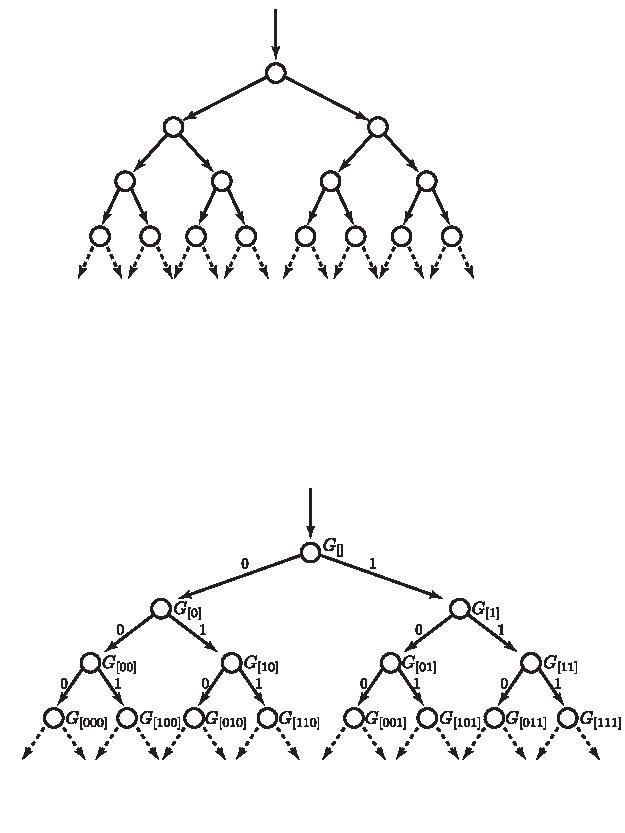
\includegraphics[trim = 4cm 8cm 4cm 8cm, clip, width=5cm]{jtfig/base.pdf}
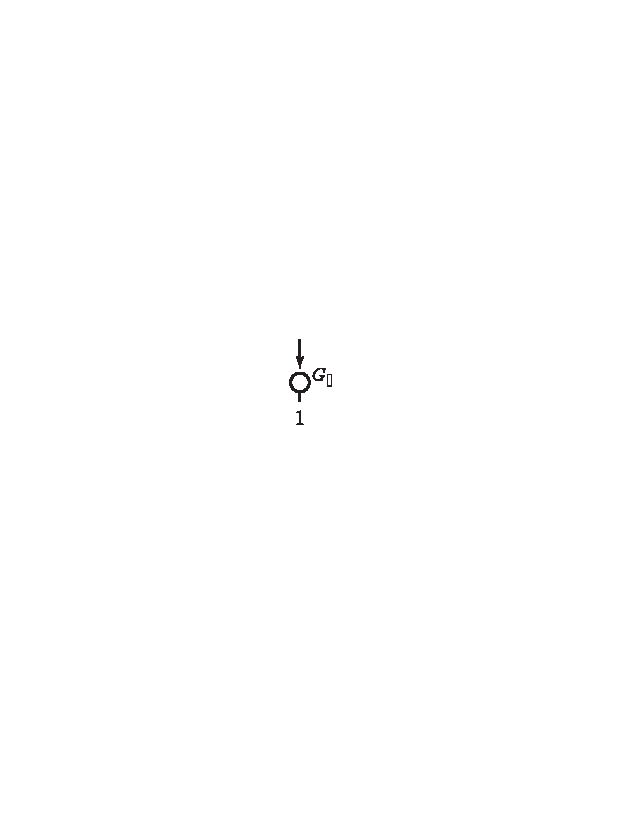
\includegraphics[trim = 2cm 2cm 2cm 6cm, width=8cm]{jtfig/seq_1.pdf}
%\caption{Test perplexity vs.~number of training observations.}
\label{fig: gm_binary_complete}
\end{center}
\end{figure}

 }
 
   \frame[t] {%slide 27
 \frametitle{Graphical Model for 110100}
 \begin{figure}[htbp]
\begin{center}
%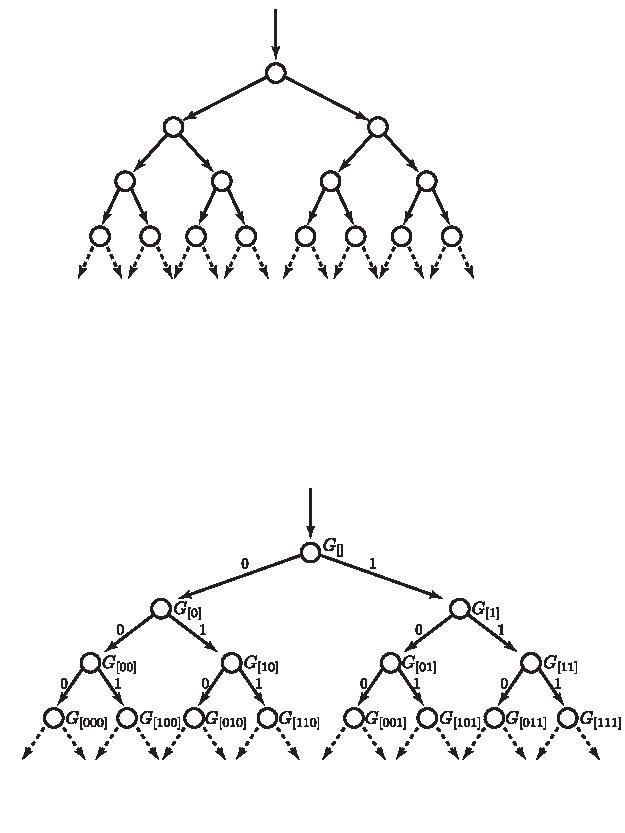
\includegraphics[trim = 4cm 8cm 4cm 8cm, clip, width=5cm]{jtfig/base.pdf}
\includegraphics[trim = 2cm 2cm 2cm 6cm, width=8cm]{jtfig/seq_2.pdf}
%\caption{Test perplexity vs.~number of training observations.}
\label{fig: gm_binary_complete}
\end{center}
\end{figure}

 }

  \frame[t] {%slide 27
 \frametitle{Graphical Model for 110100}
 \begin{figure}[htbp]
\begin{center}
%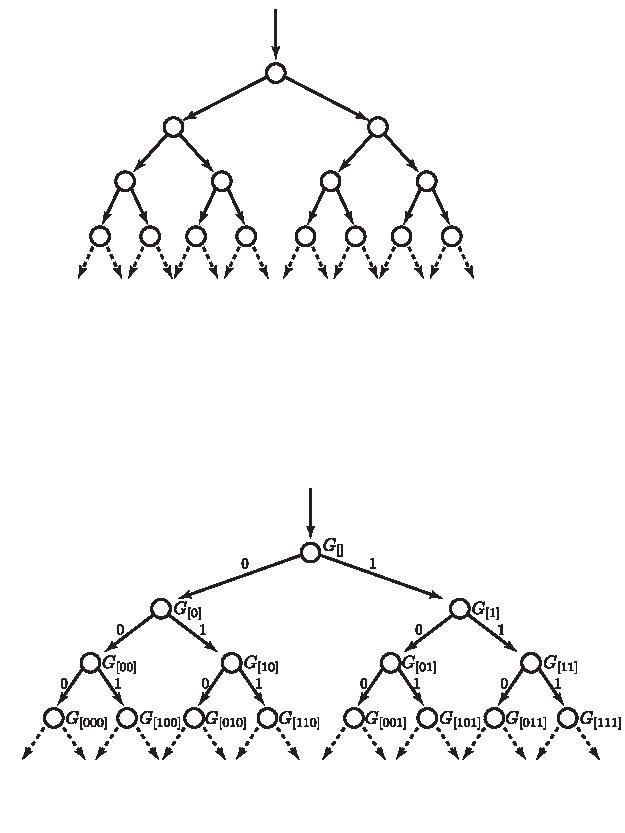
\includegraphics[trim = 4cm 8cm 4cm 8cm, clip, width=5cm]{jtfig/base.pdf}
\includegraphics[trim = 2cm 2cm 2cm 6cm, width=8cm]{jtfig/seq_3.pdf}
%\caption{Test perplexity vs.~number of training observations.}
\label{fig: gm_binary_complete}
\end{center}
\end{figure}

 }
   \frame[t] {%slide 27
 \frametitle{Graphical Model for 110100}
 \begin{figure}[htbp]
\begin{center}
%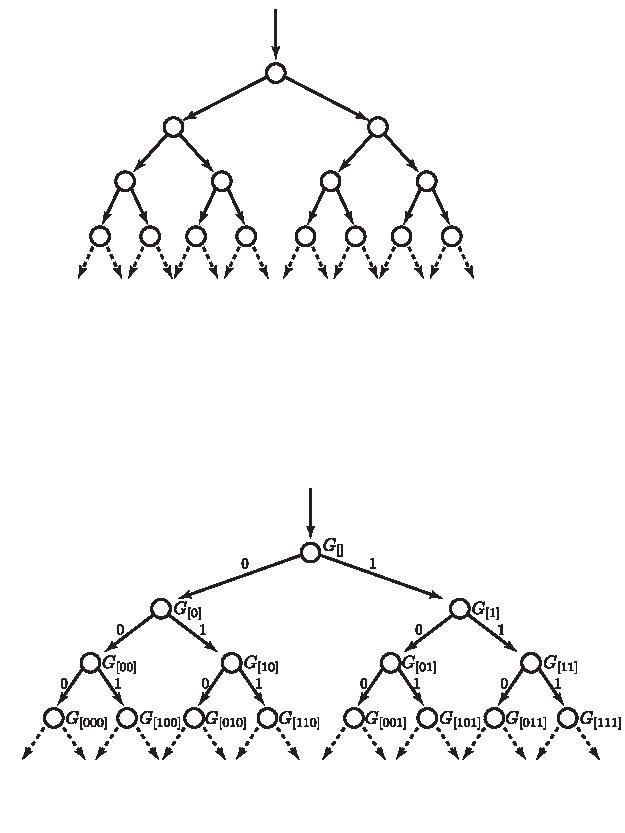
\includegraphics[trim = 4cm 8cm 4cm 8cm, clip, width=5cm]{jtfig/base.pdf}
\includegraphics[trim = 2cm 2cm 2cm 6cm, width=8cm]{jtfig/seq_4.pdf}
%\caption{Test perplexity vs.~number of training observations.}
\label{fig: gm_binary_complete}
\end{center}
\end{figure}

 }
   \frame[t] {%slide 27
 \frametitle{Graphical Model for 110100}
 \begin{figure}[htbp]
\begin{center}
%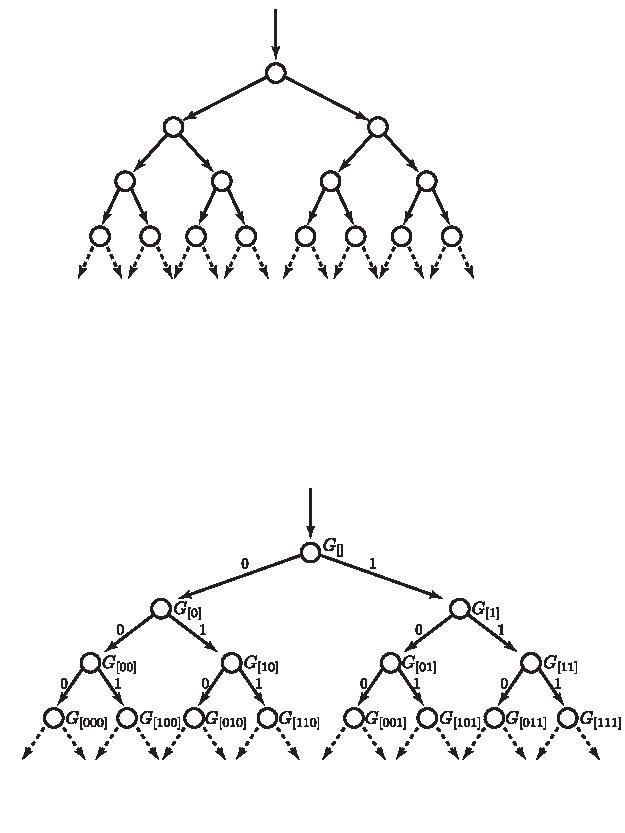
\includegraphics[trim = 4cm 8cm 4cm 8cm, clip, width=5cm]{jtfig/base.pdf}
\includegraphics[trim = 2cm 2cm 2cm 6cm, width=8cm]{jtfig/seq_5.pdf}
%\caption{Test perplexity vs.~number of training observations.}
\label{fig: gm_binary_complete}
\end{center}
\end{figure}

 }
 }
 
  \subsection{Resulting binary sequence memoizer for observed sequence 110100}
   \frame[t] {%slide 27
 \begin{figure}[htbp]
\begin{center}
%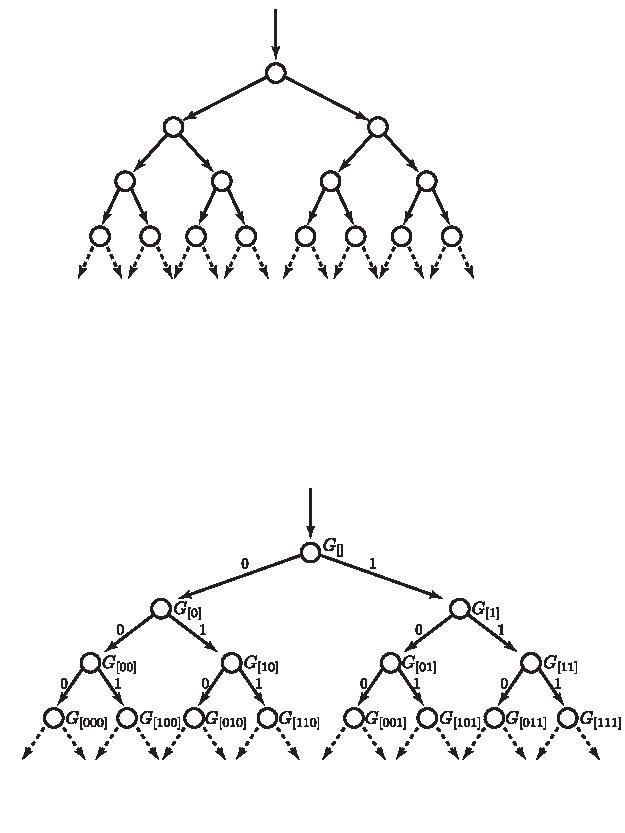
\includegraphics[trim = 4cm 8cm 4cm 8cm, clip, width=5cm]{jtfig/base.pdf}
\includegraphics[trim = 2cm 2cm 2cm 6cm, width=8cm]{jtfig/seq_6.pdf}
%\caption{Test perplexity vs.~number of training observations.}
\label{fig: gm_binary_complete}
\end{center}
\end{figure}

 }



\subsection{Inference in the sequence memoizer}
  \frame[t] {%slide 9
\[\EE[\G_\context(s)]
= \EE\left[
\frac{N(\context s)-\disc_{\context} M(\context s) + \left(\disc_{\context}\sum_{s'\in\Sigma}  M(\context s')\right) \G_\parent(s)}{\sum_{s'\in\Sigma} N(\context s')}\right]
\]
is an expectation over a set of random counts (latent variables)
\[\{N(\ubf's'),M(\ubf's')\}_{\ubf'\in\cctx, s'\in\Sigma}\]
which are subject to the constraints 
\begin{itemize}
\item  $N(\data_{1:t}x_{t+1}) \geq 1 \; \forall \; t$, observations
\item $M(\ubf's') \leq N(\ubf's')$, ``discounting''
\end{itemize}
\vspace{.5cm}
For prediction these variables are marginalized using Monte Carlo methods.
}




\section{Experiments}


\subsection{Compression of byte sequences arising from arbitrary stochastic processes (computer files)}
\frame[t]
{
\begin{block}{Performance}
\begin{table}[t]
    \begin{center}
    \setlength{\tabcolsep}{1.3mm}
\begin{tabular}{l||r|c|c|c|c}
%\hline
%\multicolumn{2}{|c||}{} & \multicolumn{2}{c||}{SM} &
%\multicolumn{2}{|c|}{PPM} & CTW\\\hline
\textbf{Model} & SM & PPM & CTW & bzip2 & gzip \\\hline
%File          &  Size  &    1PF    &    UKN    &   PPM* &    PPMZ  &  CTW  \\\hline 
%\hline
%bib           & 111261 &    1.73   &{\bf 1.72}  &   1.91 &    1.74  &  1.83 \\\hline
%book1         & 768771 &{\bf 2.17}  &    2.20   &   2.40 &    2.21  &  2.18 \\\hline
%book2         & 610856 &{\bf 1.83}  &    1.84   &   2.02 &    1.87  &  1.89 \\\hline
%geo           & 102400 &{\bf 4.40}  &    4.40   &   4.83 &    4.64  &  4.53 \\\hline
%news          & 377109 &{\bf 2.20}  &    2.20   &   2.42 &    2.24  &  2.35 \\\hline
%obj1          & 21504  &{\bf 3.64}  &    3.65   &   4.00 &    3.66  &  3.72 \\\hline
%obj2          & 246814 &    2.21   &{\bf 2.19}  &   2.43 &    2.23  &  2.40 \\\hline
%paper1        & 53161  &    2.21   &{\bf 2.20}  &   2.37 &    2.22  &  2.29 \\\hline
%paper2        & 82199  &{\bf 2.18}  &    2.18   &   2.36 &    2.21  &  2.23 \\\hline
%pic           & 513216 &    0.77   &    0.82   &   0.85 &{\bf 0.76} &  0.80 \\\hline
%progc         & 39611  &    2.23   &{\bf 2.21}  &   2.40 &    2.25  &  2.33 \\\hline
%progl         & 71646  &    1.44   &{\bf 1.43}  &   1.67 &    1.46  &  1.65 \\\hline
%progp         & 49379  &    1.44   &{\bf 1.42}  &   1.62 &    1.47  &  1.68 \\\hline
%trans         & 93695  &    1.21   &{\bf 1.20}  &   1.45 &    1.23  &  1.44 \\\hline \hline
%\textbf{avg.} &        &{\bf 2.12}  &    2.12   &   2.34 &    2.16  &  2.24 \\\hline
\textbf{Average bits / byte}      &{\bf 1.89}   & 1.93  &  1.99 & 2.11 & 2.61 \\%\hline
\end{tabular}
\end{center}
\label{table:results}
\end{table}
\end{block}
Compression performance\footnote{The results for unbounded-length context PPM is from 
\cite{Cleary1997b}. The results for CTW is from \cite{Willems2009}.   The
bzip2 and gzip results come from running the corresponding standard unix
command line tools with no extra arguments.} in terms of weighted average log-loss
\[\ell(\xbf_{1:N}) = -\frac{1}{T}\sum_{t=1}^T \log_2 \EE[G(x_t|\xbf_{1:t-1})]\]
(average bits per byte under optimal entropy encoding, lower is better) for
the Calgary corpus.


}


\subsection{Language modeling}
\frame[t]
{
\begin{block}{Performance}
 \begin{table}
\begin{center}
\begin{tabular}[t]{lcc}
\hline
{\small Source } & {\small Perplexity\footnote{perplexity = $2^{\mathrm{log\; loss}}$}} \\
\hline
{\small Bengio et al.\ \cite{Bengio2003} }& 109.0 \\
%{\small Mnih \& Hinton \cite{Mnih:NIPS08} } & 112.1 \\
{\small Mnih et al.\ \cite{Mnih2009}} & \phantom{0}83.9\\
\hline
{\small 4-gram Interpolated Kneser-Ney \cite{Chen1999} }& 106.1 \\
{\small 4-gram Modified Kneser-Ney \cite{Chen1999} }& 102.4 \\
{\small 4-gram Hierarchical PYP \cite{Teh2006} } & 101.9 \\
{\small Sequence Memoizer} \cite{Wood2009}& \phantom{0}96.9\\
\hline
\end{tabular}
\end{center}
 %It has
 %been reported that the aspects of the data that are modelled by these two
 %distinct classes of models complement each other, so that even higher perfomance
 %can be achieved by combining both types of models.
 % The sequence memoizer outperforms fixed depth smoothing $n$-gram models but is bettered by a more computationally complex model on this data.  }
\label{table:ap_perplexities}
\end{table}
\end{block}
{\small Language models of an antagonistically processed Associated Press news corpus (lower perplexity is better).  Interpolated and
 modified Kneser-Ney are state-of-the-art language models.  Provided for comparison are 
 the results for the models of Bengio et al.\ and Mnih et al.\ which belong to
 a different class of models that learn word representations from data. }
}

\subsection{Finite order Markov models vs. the sequence memoizer}
\frame[t]
{
\begin{figure}
    \includegraphics[width=.85\columnwidth]{cacm_figs/lm_results}
    \label{fig:sm_vs_ngram}
\end{figure}
 SM  versus $n^{\textrm{th}}$ order Markov models
%    $n$-gram model (solid line)
    as $n$ varies.  In red is computational
    complexity. % (for both the sequence 
%    memoizer (dashed line) and a smoothing $n$-gram model (solid line).
    %For this four million word New York Times corpus, as $n$ passes 4, the memory complexity of the Markov models grows larger than that of the sequence
   % memoizer, yet, the SM model yields modeling
   % performance that is better than all Markov models regardless of their order. %the limit of an $n$-gram as $n\rightarrow\infty$.
  %  This suggests that for $n\ge 4$ the SM model is to be preferred: it
  %  requires less space to store yet results in a comparable if not better
  %  model.
}



\section{Improvements}
\subsection{Incremental Estimation}
\begin{frame}[t]{}
Incremental estimation (particle filter), \citet{Gasthaus2010}.  
\begin{itemize}
\item First scalable implementation 100's MB's (Wikipedia 1.66 bits/byte, 100MB $\rightarrow$ 20.8MB, outperformed by PAQ)
\item 4.35 bits per Chinese character (better than best reported result of 5.44 bits \cite{Wu2007}).
\end{itemize}

\vspace{2cm}

Still $\Omega(N)$ storage complexity.

%1-PF and Kneser-Ney variant approximately equal.

\end{frame}

\subsection{Constant space approximate inference}
\begin{frame}[t]{}
\begin{block}{``Forgetting counts,'' \citet{Bartlett2010}}
\begin{figure}[htbp]
\begin{center}
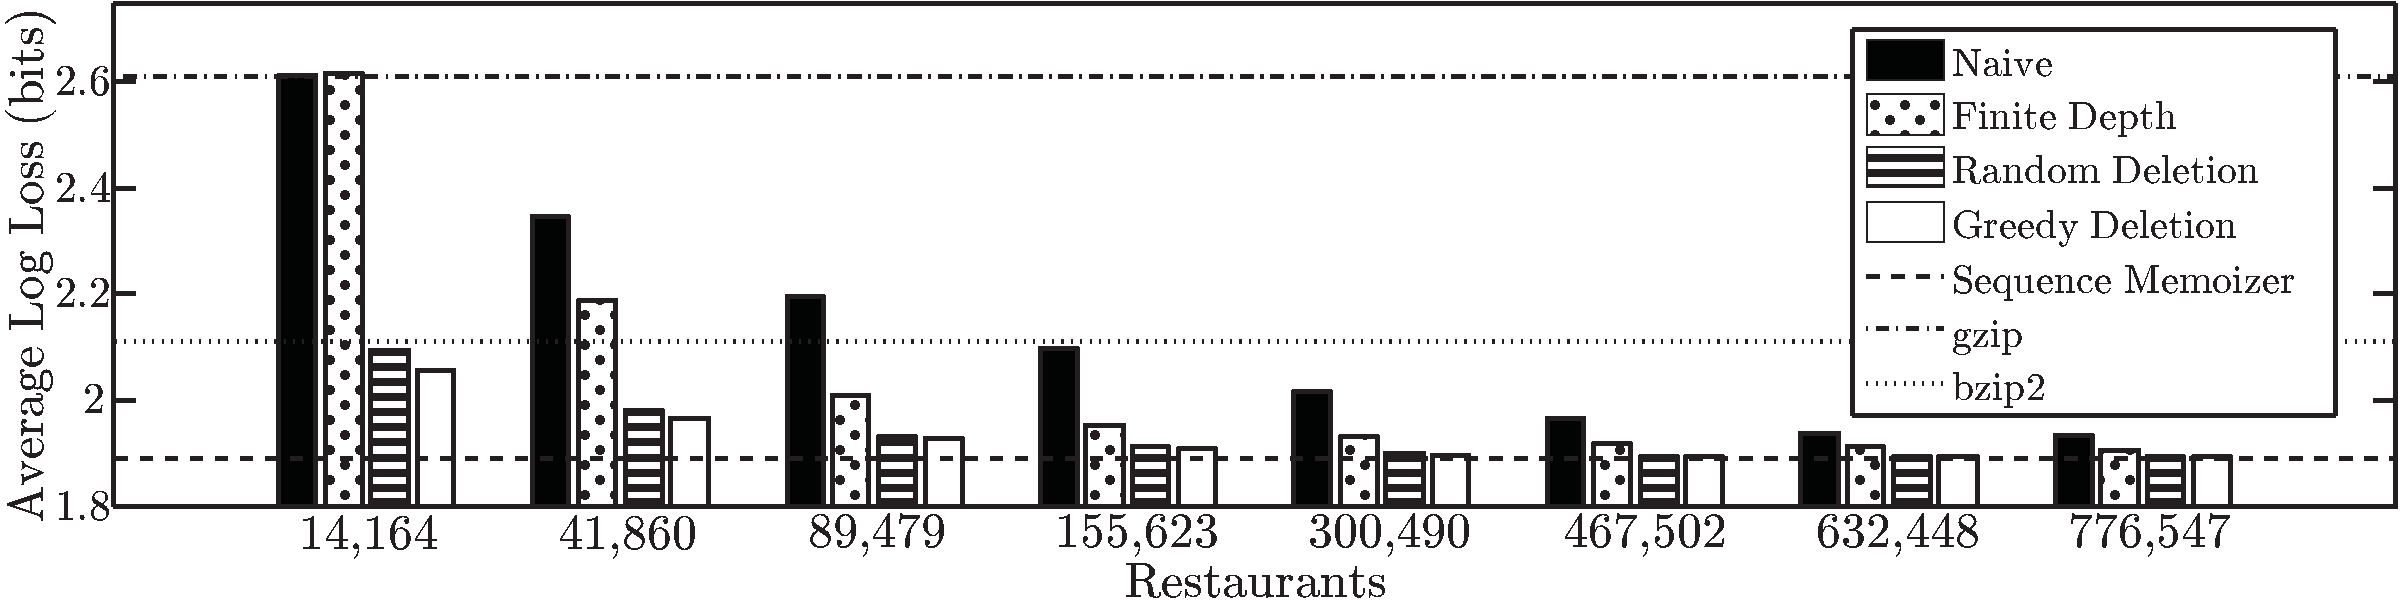
\includegraphics[width=\textwidth]{results_calgary_corpus.pdf}
\end{center}
\end{figure}
A dependent HPYP can be defined though a graphical model leaf node deletion scheme.  Inference in the resulting model was shown to approximate the SM well.  \tiny{data: Calgary corpus, rests = total used nodes in 3-10 grams}
\end{block}
\begin{block}{``Improvements to the sequence memoizer,'' \cite{Gasthaus2011}}
Only $O(2|\Sigma|)$ numbers need be stored for each node in the SM graphical model.
\end{block}

\end{frame}

\subsection{``Deplump for Streaming Data'' \citet{Bartlett2010}, Constant space, constant time prediction, linear time estimation SM}
\begin{frame}[t]{}
%\begin{block}{}
%\begin{figure}[htbp]
%\begin{center}
%\includegraphics[width=\textwidth]{varying_depths.pdf}
%\end{center}
%\end{figure}
%A dependent HPYP can be defined though a graphical model leaf node deletion scheme.  Inference in the resulting model was shown to approximate the SM well.  \tiny{data: Calgary corpus, rests = total used nodes in 3-10 grams}
%\end{block}
\begin{figure}[htbp]
\begin{center}
\includegraphics[width=\textwidth]{varying_stream_length.pdf}
\end{center}
\end{figure}
First streaming SM with computational asymptotics required for streaming compression.  Compressed 26.8Gb Wikipedia corpus to 4Gb (vs. 7.9Gb for gzip and 3.8Gb for PAQ).\newline
\vspace{3cm}
{\tiny $L$ is number of nodes in SM, data Wikipedia dump 2010 head, depth 16}
\end{frame}


%\subsection{Roadmap of sequence memoizer literature}
%\begin{frame}[t]{}
%Linear space sequence memoizer (SM)
%\begin{itemize}
%\item ``A Stochastic Memoizer for Sequence Data'' \cite{Wood2009}
%\item ``The Sequence Memoizer'' \cite{Wood2011}
%\end{itemize}
%SM inference
%\begin{itemize}
%\item ``A Bayesian Interpretation of Interpolated Kneser-Ney'' \citet{Teh2006}
%\item ``Hierarchical Dirichlet processes'' \cite{Teh2006b}
%\item ``A Hierarchical {B}ayesian Language Model based on {P}itman-{Y}or Processes'' \cite{Teh2006a}
%\item ``Gibbs Sampling Methods for Stick-Breaking Prior'' 



%\cite{Ishwaran2001a}
%\end{itemize}
%Constant space SM
%\begin{itemize}
%\item ``'Forgetting Counts : ... '' \cite{Bartlett2010}
%\item ``Improvements to the Sequence Memoizer'' \cite{Gasthaus2011}
%\end{itemize}
%Incremental inference
%\begin{itemize}
%\item ``Lossless compression based on the {S}equence {M}emoizer'' \cite{Gasthaus2010}
%\item ``Streaming Deplump'' \cite{Bartlett2011}
%\end{itemize}

%\end{frame}

\section{Beyond}
\subsection{A path to better models of the ``world''}
\frame[t]
{
\begin{itemize}
\item Introduce more degrees of freedom into the model (?)
%\item Develop nonparametric variants of models with greater expressivity in the automata theory (recognizability) / formal grammar sense (generative)
%\item Decouple states of the world from conditional emission distributions
\item Try to {\em learn} a small set of frequently reused states and share strength between them.
\item Requires mapping more than one context to each state.
\end{itemize}
}


\subsection{Generalizing from Markov models to PDFA }
\frame[t]
{
\begin{center}
Automata corresponding to binary $1^{\mathrm{st}}$-order Markov model
\end{center}
\begin{figure}
    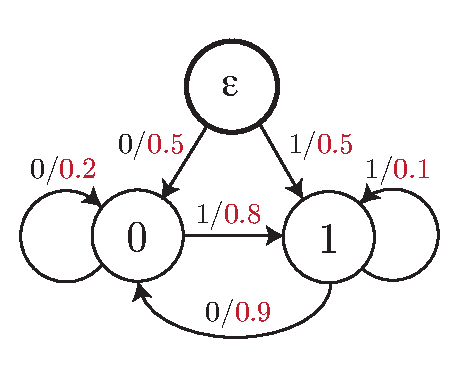
\includegraphics[width=.5\columnwidth]{bigram}
    \label{fig:bigram}
\end{figure}

\begin{itemize}
\item {\em Probabilistic deterministic finite automata} capable of {\em recognizing} and {\em generating} arbitrary binary sequences.
\item A Markov model is an automata with defined, deterministic transition function and corresponding set of states.
\end{itemize}

}

\frame[t]
{
\begin{center}
Automata with no corresponding finite-order Markov model
\end{center}
\begin{figure}
    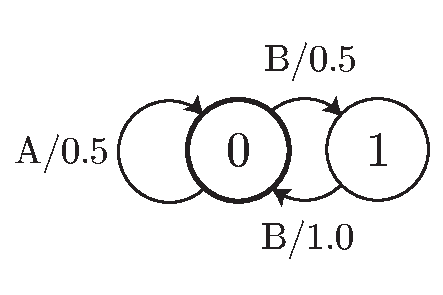
\includegraphics[width=.5\columnwidth]{even}
    \label{fig:even}
\end{figure}
\begin{itemize}
\item {\em Even process} can generate ABBA, AAABBBBABB, BBBBBBBB, but not ABA.
\item Many contexts correspond to the the same state.
\item Learnable using frequentist tools \cite{Carrasco1994,Thollard2000,Shalizi2004}
\end{itemize}
}

\subsection{Probabilistic Deterministic Infinite Automata, \citet{Pfau2010}}
\frame[t]
{
 A Probabilistic Deterministic Infinite Automata (PDIA) is a Bayesian nonparametric limit of a PDFA with an unbounded number of states.  Formally a PDIA is a quintuple 
 \[M = (Q,\Sigma,\delta,\{\vec{\pi}_i\},q_0)\]
  where
  \begin{itemize}
\item $Q$ is a countable set of states
\item $\Sigma$ is a finite set of symbols
\item $\delta: Q \times \Sigma \rightarrow Q$ is a deterministic transition function from state/symbol pairs to another state
\item $\{\vec{\pi}_i : i \in Q\}$ is a set of probability vectors over symbols, one for each state
\item $q_0$ is the initial state
\end{itemize}
}

\frame[t]
{
One possible PDIA prior
 \begin{eqnarray*}
G_0 &\sim& \PY(\gamma,d_0,H) \\
G_\sigma &\sim& \PY(\alpha, d, G_0) \\
\delta(q_i,\sigma) &\sim& G_\sigma \\
\vec{\pi}_i &\sim& \mathrm{Dir}(\beta/|\Sigma|,\ldots,\beta/|\Sigma|)
\end{eqnarray*}
given a sequence $\bx$ a posterior over
 \[\mathcal{H} = \{\delta,\{\vec{\pi}_i\}\}\]
 can be learned from data and used for prediction
 \[P(x_T |\data) = \int P(x_T | \mathcal{H} ) P(\mathcal{H}  | \data) dP(\mathcal{H})\]
}

\frame[t]
{
Key points
\begin{itemize}
\item World states are {\em learned} from data. 
\item  Prior biases towards a state re-use.
\item State-to-state transitions learned from data.
\item States not identifiable by context.
%\item Because of deterministic transitions, forward prediction is still extremely fast.
\end{itemize}
}

\subsection{PDIA Performance}
\frame[t]
{
\begin{table}[t]
    \begin{center}
    \setlength{\tabcolsep}{1.3mm}
    \begin{small}
\begin{tabular}{r|cccccccccc}
\hline
& SM  & PDIA  &  HMM \\
\hline
AIW & 4.78 & 5.13  &  7.89   \\
  & 19,358 & 365.6 & 52   \\
\hline
\hline
%AIWL & 4.08 & 4.13 &  7.89 & 9.45 & 5.72 & 4.05 & 3.51 & 3.32 & 3.24 \\
 %AIWL & 1,231.6 & 1,247 &  52 & 28 & 444 & 3,249 & 12,324 & 31,990 & 177,232 \\
%\hline
%\hline
DNA & 3.56 & 3.72  &  3.76   \\
 & 314,166 & 64.7  & 19   \\
\hline
\end{tabular}
\end{small}
\end{center}
%\vspace{-8mm}
\end{table}
{\small Evaluation on Alice in Wonderland (AIW) and mouse DNA.  Top row is perplexity of test set, bottom is number of states in the model (average for PDIA).  PDIA: average over multiple posterior samples. HMM: Hidden Markov Model.  SM: sequentially trained sequence memoizer.}\newline

\vspace{.5cm}
HMM arises when $\delta$ not deterministic.
}



\subsection{Some of the many things I don't understand}
\frame[t] {
For a fixed length, real-world observation sequences, we've found that the empirical predictive performance of {\em Bayesian} models that bias towards more compact representations of the world (fewer states) is often {\em worse} than models that carefully estimate emission distributions for more states.  
\begin{itemize}
\item Is Bayesian inference in broken?
\begin{itemize}
\item Does posterior ``search'' need to be improved?
\item Do ``smoother'', easier to traverse priors need to be defined? 
\end{itemize}
\item Is the bias too strong?
\item Do we simply need more data?  
\item Are we selecting the wrong states?
\item Is predictive performance the wrong measure?
\end{itemize}

}

\subsection{Questions that keep me awake at night}
\frame[t]
{
\begin{itemize}
\item Nonparametric estimators fundamentally have the wrong storage asymptotics.    
\begin{itemize}
\item Should we abandon them?
\item Is the class of parametric estimators derived nonparametric estimators for ``compacted'' nonparametric models interesting?
\item Is there a provable advantage to or optimal strategy for forgetting in counting models?
\end{itemize}
\item How do we distinguish between the expressivity of models of infinite complexity?  
\item How do we learn $\sigma$, or, more generally, how to we compute in a model with countable back-offs?
\item What happens when the input vocabulary gets very big and the typical input vector is high-dimensional?
%All models can generate (place mass on) all strings, so is this a rate of convergence problem?  What about unknown stochastic processes?
\end{itemize}
}

\subsection{Take Home}
\frame[t]{
\begin{itemize}
\item Sequence Memoizer and PDIA are fundamentally new Bayesian nonparametric models
\begin{itemize}
\item Both are ``inefficient'' models of the world but {\em perform} very well as predictors.
\end{itemize}
\item SM is a computationally tractable $\infty$-order drop-in replacement for $n^{\mathrm{th}}$-order Markov models
\item Deplump is a good, general purpose compressor, built on the constant space/time sequence memoizer.
\item SM  ($\approx$ 1.4 bits/character) approaches {\em human} ($\approx$ 1 bits/character) predictive performance for written English.
\item Bayesian nonparametric discrete sequence models, show promise as the foundation for general purpose predictors.
\end{itemize}

}

\section{Demo}
\subsection{Compressor based on the sequence memoizer}
\frame[t]
{
A general purpose streaming lossless compressor (``deplump'') built on the sequence memoizer  is available for demonstration at
  \begin{itemize}
  \item \href{http://www.deplump.com/}{http://www.deplump.com/} 
  \begin{itemize}
\item    \href{http://www.deplump.com/LookupStatistics}{real time performance} 
\end{itemize}
\end{itemize}
Source code for the sequence memoizer is downloadable from 
\begin{itemize}
  \item  \href{http://www.sequencememoizer.com/}{http://www.sequencememoizer.com/} 
  \end{itemize}
}



%\section{References}

\subsection{Bibliography}
\bibliographystyle{plainnat}
	\begin{frame}[t,allowframebreaks]{}

\bibliography{../../papers/uber}
\end{frame}


%\subsection{Data: one complicated stochastic process exhibiting recency and power-law characteristics}
\begin{frame}[t]{}
\begin{figure}[t]
    \begin{center}
        \includegraphics[width=.75\columnwidth]{cacm_figs/powerlaw/freq_plot}
    \end{center}
    \label{fig:powerlaw}
\end{figure}
Power-law scaling of word frequencies in
    English text. Relative word frequency  is plotted against each words' rank when ordered according to
    frequency. There are a few very common words and a large
    number of relatively rare words. \\ {\tiny Figure from \cite{Wood2011}}.
\end{frame}	

\frame[t]{
Many nonparametric Bayesian models have been designed.\newline

Automata
\[  \mbox{Finite} \subset \mbox{Non-deterministic pushdown} \subset \mbox{Turing machine} \]
Corresponding Bayesian nonparametric models\\
\begin{center}
\small
SM \cite{Wood2009} $\sqsubset$ PDIA \cite{Pfau2010} $\sqsubset$ IHMM \cite{Beal2002}  $\subset$ IPCFG \cite{Johnson2007,Liang2007} $\subset$ Church \cite{Goodman2008} $\sqsubset$ \cite{Liang2010} 
\end{center}
Making them work well and understanding their characteristics is an open problem. 
}

%\subsection{An aside: stochastic memoization}
\begin{frame}[t]{}
A stochastic memoizer \cite{Goodman2008} is a non-deterministic function cache 
\begin{align*}
SM(\context) = \left\{\begin{array}{ccc}
\sigma_1  & \mbox{w.p.}  &  G_\context(\sigma_1) \\
\sigma_2  & \mbox{w.p.}  &  G_\context(\sigma_2)  \\
  &  \vdots &   
\end{array}\right.
\end{align*}
with $\sigma_i \in \Sigma$.
\vspace{.5cm}

Posterior inference in many Bayesian nonparametric models can be described in terms of stochastic memoization. 
\end{frame}

\begin{frame}[t]{}
Posterior inference in the sequence memoizer is hierarchical stochastic memoization of sequence continuations. 
\begin{align*}
SM(\context) = \left\{\begin{array}{ccc}
\sigma_1  & \mbox{w.p.}  &  \EE[G_\context(\sigma_1)] \\
\sigma_2  & \mbox{w.p.}  &  \EE[G_\context(\sigma_2)]  \\
  &  \vdots &   
\end{array}\right.
\end{align*}
with $\sigma_i \in \Sigma$.
\vspace{.5cm}
\end{frame}

\end{document}
